\chapter{Analiza cerințelor și motivație}

\section{Motivație}
Decizia de a construi această platformă a pornit de la o observație concretă legată de modul în care oamenii studiază limba engleză online, majoritatea utilizatorilor care doresc atât materiale de studiu structurate, cât și posibilitatea de a lucra direct cu un profesor ajungând să folosească servicii diferite pentru fiecare dintre aceste nevoi, fără ca ele să fie integrate în vreun fel. Fragmentarea aceasta are consecințe practice directe, progresul acumulat pe o platformă nefiind vizibil pe cealaltă platformă, profesorul neavând cum să știe ce a studiat studentul până în acel moment și neputând adapta sesiunea în funcție de nivelul real al acestuia, iar costul combinat al mai multor abonamente devenind un factor descurajant în timp.

Pentru a valida această observație, a fost realizat un sondaj în cadrul proiectului, la care au participat 28 de persoane, urmărind înțelegerea obiceiurilor și nevoilor utilizatorilor în studiul limbii engleze online, rezultatele confirmând fragmentarea descrisă. La întrebarea privind modul în care accesează materialele de studiu și sesiunile cu un profesor, 16 din 28 de respondenți au indicat că le accesează prin servicii separate, 9 au menționat că folosesc exclusiv una dintre variante, iar doar 3 au indicat că le găsesc în aceeași platformă (\Cref{fig:survey-q04}), confirmând că nevoia de integrare este reală pentru majoritatea utilizatorilor chestionați.

La întrebarea dacă ar folosi o platformă care combină cursuri structurate, exerciții și sesiuni video cu profesori verificați, 25 din 28 de participanți s-au declarat interesați de o soluție integrată, 15 cu certitudine și 10 indicând ca ar folosi-o cel mai probabil, în timp ce doar 3 au răspuns negativ (\Cref{fig:survey-q07}), indicând o cerere clară pentru un astfel de sistem și constituind principala justificare pentru realizarea platformei. Rezultatele complete ale sondajului, incluzând distribuția răspunsurilor pentru toate cele opt întrebări, sunt disponibile în Anexa A pentru consultare detaliată.

\begin{figure}[htbp]
    \centering
    \begin{subfigure}{0.48\textwidth}
        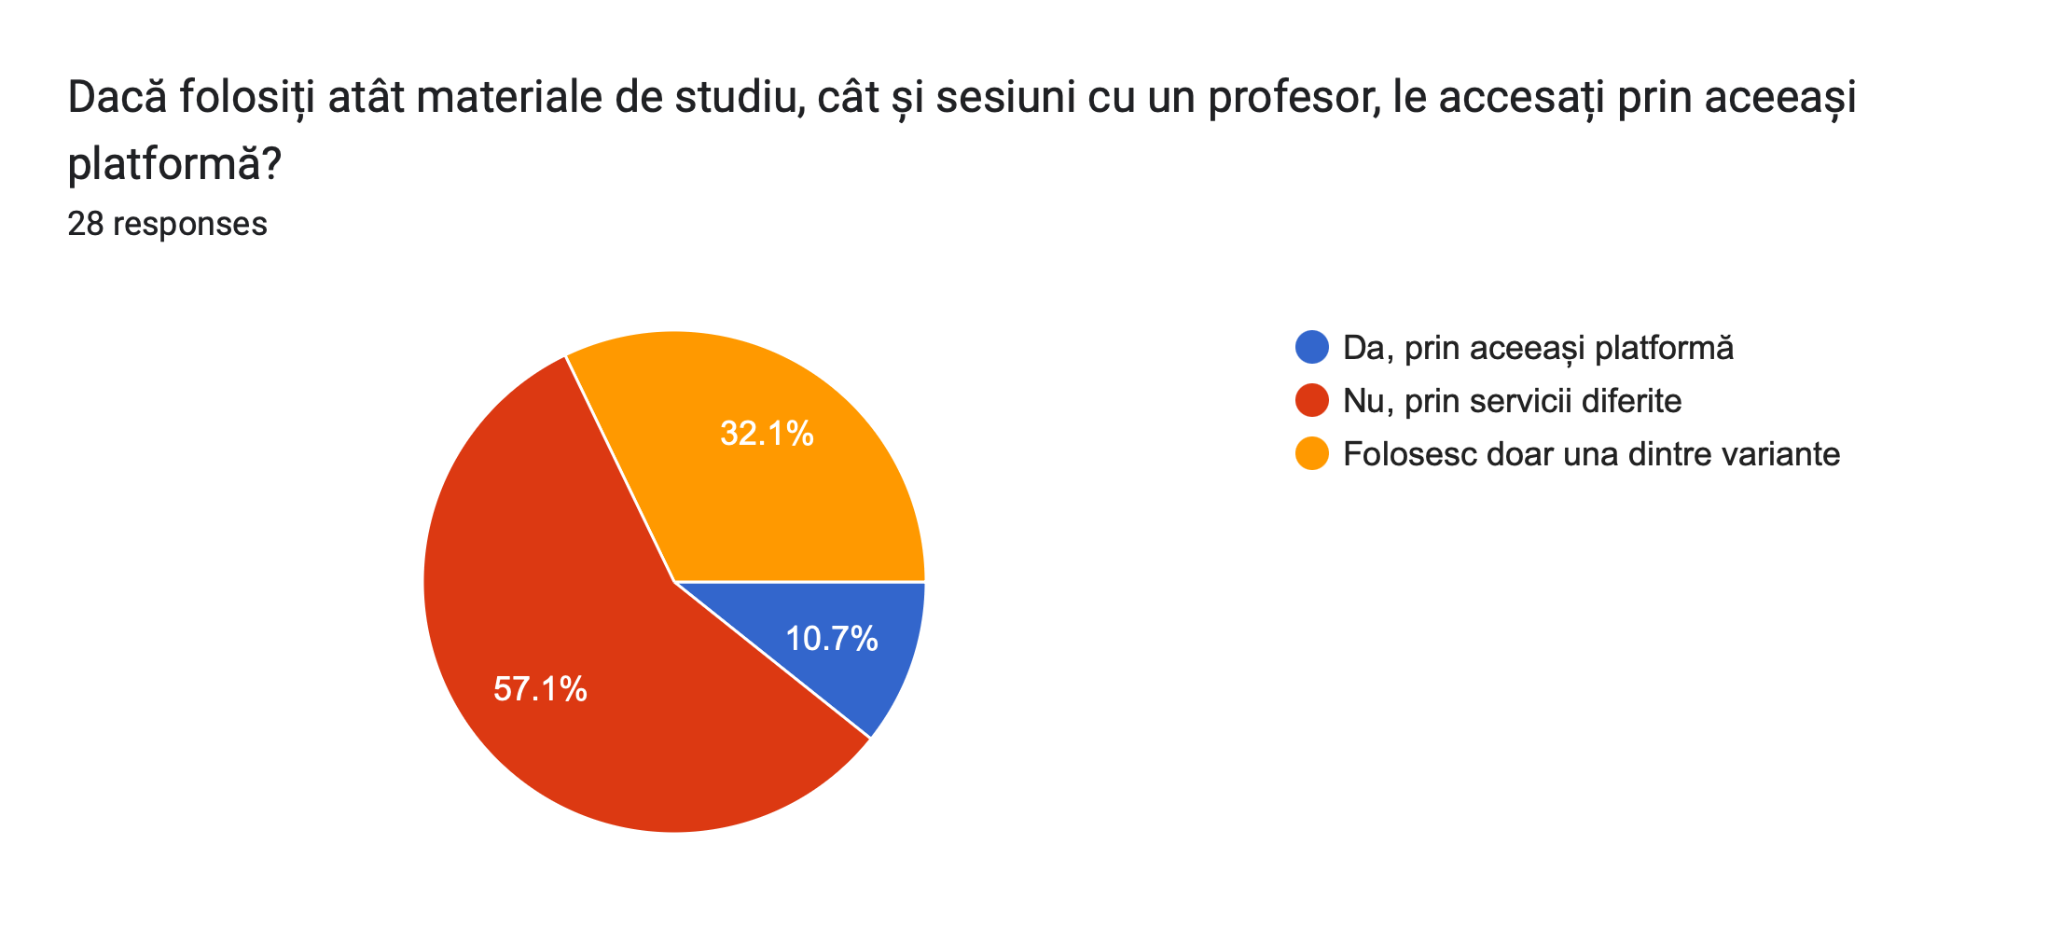
\includegraphics[width=\textwidth]{pics/survey/q04.png}
        \caption{Distribuția modului de acces la materiale de studiu și sesiuni cu un profesor}
        \label{fig:survey-q04}
    \end{subfigure}
    \hfill
    \begin{subfigure}{0.48\textwidth}
        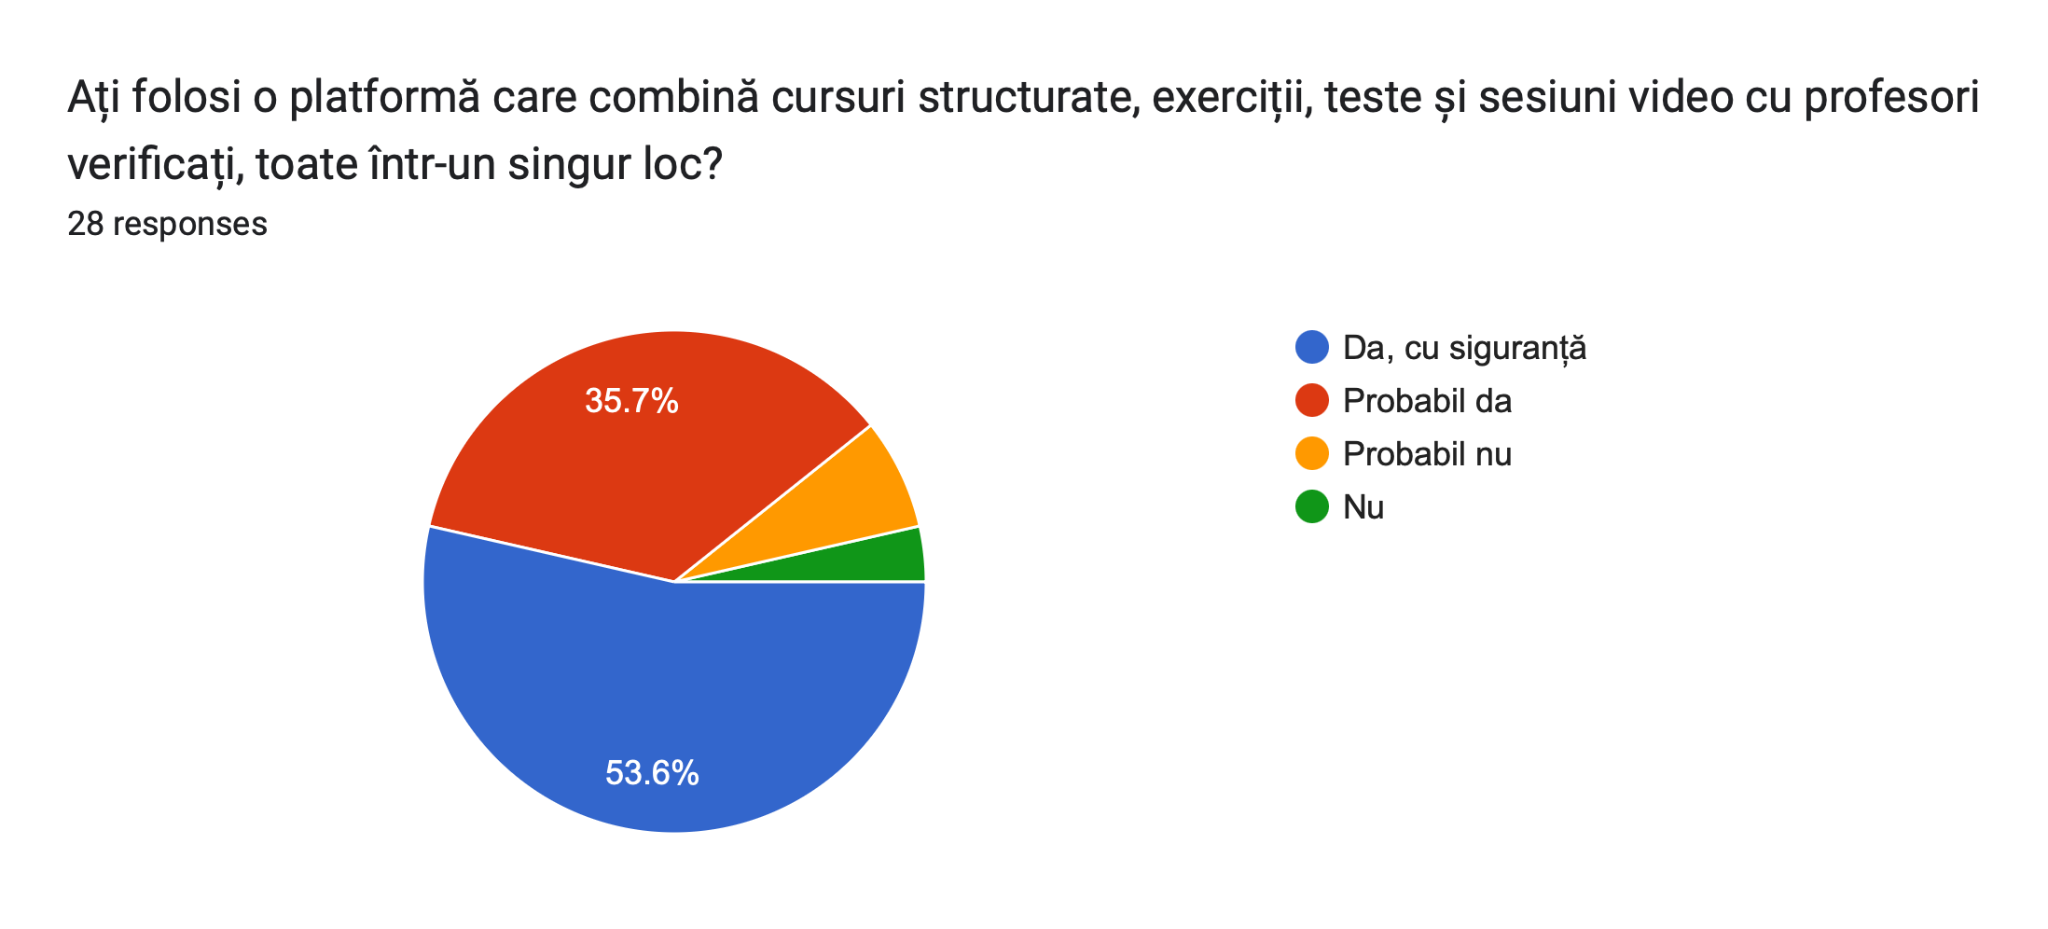
\includegraphics[width=\textwidth]{pics/survey/q07.png}
        \caption{Interesul față de o platformă care integrează materiale de studiu și sesiuni cu profesori}
        \label{fig:survey-q07}
    \end{subfigure}
    \caption{Nevoia de integrare a serviciilor de învățare}
\end{figure}

Nevoia de integrare este susținută și din perspectivă academică, studiul realizat de Tao et al. demonstrând că abordarea combinată, îmbinând studiul individual cu interacțiunea directă cu un profesor, are un impact pozitiv semnificativ asupra competenței în limba engleză față de metodele bazate exclusiv pe studiul individual, studenții care au urmat cursuri bazate pe această abordare înregistrând progrese măsurabile la nivelul tuturor abilităților evaluate \cite{eobtocs_efl_a2024}. Concluzia studiului susține ideea că niciuna dintre cele două componente nu poate asigura singură un progres optim, combinarea lor ducând la rezultate semnificativ mai bune și justificând astfel decizia de a le integra pe ambele într-un singur sistem.

\section{Cerințe de sistem}
Din punctul de vedere al cerințelor de sistem, platforma rulează direct în browser fără a fi necesară instalarea vreunei aplicații separate, singurele condiții tehnice fiind un browser modern și o conexiune stabilă la internet, cerințe pe care orice dispozitiv modern le îndeplinește fără configurări suplimentare.

\section{Categorii de utilizatori}
Platforma este organizată în jurul a trei roluri principale, fiecare cu un set distinct de funcționalități și restricții, accesul la diferite secțiuni ale sistemului fiind condiționat de rolul pe care îl deține utilizatorul și verificat automat la fiecare cerere adresată serverului.

Studentul este utilizatorul principal al platformei, scopul său fiind acela de a studia limba engleză parcurgând materialele disponibile în catalog și interacționând cu profesorii înregistrați în platformă prin sesiuni video, accesul la funcționalitățile platformei fiind condiționat de existența unui cont activ, creat în urma unui proces de verificare prin email. Utilizatorii minori necesită și obținerea consimțământului parental înainte de activarea contului.

Profesorul are un rol dual pe platformă, putând crea conținut educațional și desfășura sesiuni video cu studenții. Accesul la funcționalitățile specifice acestui rol nu este disponibil imediat după înregistrare, ci condiționat de aprobarea unei cereri de activare din partea administratorului, asigurând astfel un nivel minim de verificare a calificărilor înainte de orice interacțiune cu studenții înregistrați.

Administratorul are acces complet la toate entitățile din sistem, rolul său fiind acela de a gestiona utilizatorii, de a valida profesorii și conținutul creat de aceștia și de a menține calitatea generală a platformei, neparticipând el însuși la conținutul didactic, ci coordonând funcționarea întregrului sistem din perspectivă administrativă.

\section{Cerințe funcționale}
Cerințele funcționale ale platformei sunt organizate în jurul celor trei roluri principale și derivă din analiza problemei identificate și din rezultatele sondajului realizat în cadrul proiectului.

\textbf{Cerințele rolului „Student”}

\begin{figure}[htbp]
    \centering
    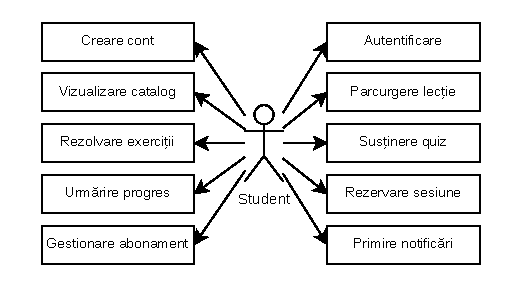
\includegraphics[width=0.8\textwidth]{pics/diagrams/usecase-student.pdf}
    \caption{Diagramă de cazuri de utilizare: Student}
    \label{fig:usecase-student}
\end{figure}

Studentul poate crea un cont completând adresa de email, parola și alte date personale de bază, contul nedevenind activ imediat, ci necesitând confirmarea adresei de email prin accesarea unui link trimis automat de sistem, prevenind astfel înregistrarea cu adrese invalide sau nedeținute de utilizator. În cazul utilizatorilor minori, platforma solicită suplimentar acordul unui părinte sau tutore legal, trimițând o cerere la o adresă de email specificată la înregistrare și activând contul doar după primirea acestui acord, asigurând conformitatea cu cerințele de protecție a datelor pentru persoanele sub 18 ani. Odată autentificat, studentul poate accesa catalogul de cursuri organizate pe trei niveluri de dificultate, parcurgând lecțiile și rezolvând exercițiile interactive asociate fiecăreia, acestea putând fi de mai multe tipuri, incluzând întrebări cu variante de răspuns, completare de spații libere și răspunsuri scurte, fiecare tip de exercițiu evaluând abilități diferite ale studentului.

Marcarea unei lecții ca finalizată este condiționată de rezolvarea corectă a exercițiilor asociate acesteia, platforma asigurându-se astfel că studentul a înțeles conținutul prezentat înainte de a putea avansa, prevenind situația în care acesta ar trece mai departe fără a demonstra că a asimilat informațiile. Pe lângă exerciții, fiecare curs poate conține quiz-uri cronometrate, studentul trebuind să răspundă la toate întrebările în intervalul de timp stabilit de profesor, testul trimițându-se automat la expirarea timpului cu răspunsurile completate până în acel moment. Progresul este urmărit automat la nivel de lecție și de quiz pentru fiecare curs, studentul putând vizualiza oricând câte lecții a finalizat, cate quiz-uri a trecut și un procent general de completare, oferindu-i o imagine clară a evoluției sale fără a fi nevoit să țină singur evidența.

Accesul la sesiunile cu profesori este condiționat de existența unui sold de credite, pe care studentul le poate obține fie printr-un abonament lunar, fie prin achiziționarea lor separată, folosindu-le ulterior pentru rezervări individuale sau de grup în funcție de disponibilitatea profesorilor și de preferința sa, tipul sesiunii influențând numărul de credite deduse. Creditele sunt deduse automat la momentul rezervării, studentul putând consulta oricând istoricul tranzacțiilor și gestiona sau anula abonamentul printr-un portal dedicat, fără a fi necesară intervenția administratorului. De asemenea, studentul primește notificări în aplicație pentru evenimente relevante, cum ar fi confirmarea unei rezervări, remindere înainte de sesiunile programate sau modificări ale conținutului la care are acces (\Cref{fig:usecase-student}).

\textbf{Cerințele rolului „Profesor”}

\begin{figure}[htbp]
    \centering
    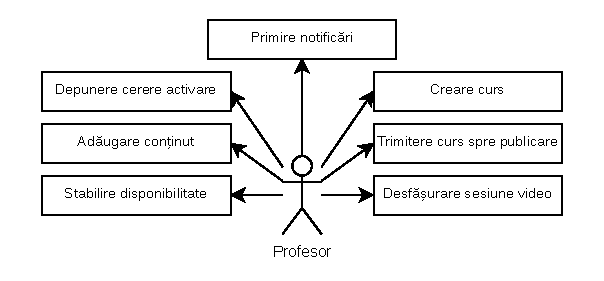
\includegraphics[width=0.8\textwidth]{pics/diagrams/usecase-professor.pdf}
    \caption{Diagramă de cazuri de utilizare: Profesor}
    \label{fig:usecase-professor}
\end{figure}

După crearea contului, profesorul depune o cerere de activare trimisă spre analiză administratorului, neavând acces la funcționalitățile specifice rolului până la aprobare. În cazul respingerii, acesta primește o notificare cu motivul deciziei, putând depunde o nouă cerere după efectuarea modificărilor necesare. Odată aprobat, profesorul poate crea cursuri noi specificând titlul, descrierea și nivelul de dificultate, adăugând lecții cu exerciții interactive de diferite tipuri și quiz-uri cu limită de timp configurabilă, cursurile rămânând în stare de draft până la trimiterea spre publicare și putând fi editate și completate oricând în această perioadă, fără a fi vizibile studenților. La trimiterea spre publicare, cursul intră automat într-un flux de revizuire gestionat de administrator, devenind vizibil în catalog doar după aprobare, profesorul primind o notificare cu decizia luată și, în cazul respingerii, cu observațiile adăugate de administrator.

Profesorul configurează intervalele orare în care este disponibil pentru sesiuni, specificând zilele și orele, sistemul generând automat sloturile disponibile pe baza acestor configurații, ca mai apoi să le afișeze studenților la momentul rezervării, astfel încât aceștia să poată alege un interval potrivit fără a fi nevoie de comunicare directă prealabilă. La momentul sesiunii, profesorul accesează camera video direct din interfața platformei, întreaga interacțiune desfășurându-se fără a fi necesară deschiderea unei aplicații externe, asigurând o experiență unitară în cadrul sistemului. Profesorul este notificat când un student rezervă o sesiune și când administratorul ia o decizie cu privire la un curs trimis spre publicare, putând vedea și eventualele observații adăugate în cazul respingerii, pe care le poate folosi pentru a îmbunătăți conținutul și a-l retrimite (\Cref{fig:usecase-professor}).

\textbf{Cerințele rolului „Administrator”}

\begin{figure}[htbp]
    \centering
    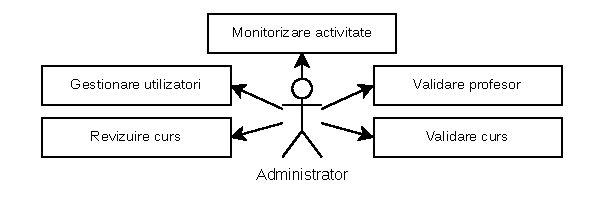
\includegraphics[width=0.8\textwidth]{pics/diagrams/usecase-admin.pdf}
    \caption{Diagramă de cazuri de utilizare: Administrator}
    \label{fig:usecase-admin}
\end{figure}

Administratorul poate vizualiza toți utilizatorii din sistem și poate gestiona conturile acestora, inclusiv să suspende sau să reactiveze un cont în situațiile care impun intervenția sa, având astfel control complet asupra accesului în platformă. Cererile de activare depuse de profesori sunt analizate de administrator, care poate aproba sau respinge fiecare cerere, profesorul primind o notificare automată cu decizia luată și, în cazul respingerii, cu motivul aferent, putând astfel înțelege ce modificări sunt necesare înainte de a depune o nouă cerere. Cursurile trimise de profesori spre publicare intră automat în coada de revizuire a administratorului, care poate aproba publicarea în catalog sau le poate respinge adăugând note cu observațiile sale, vizibile profesorului și utile pentru corectarea conținutului, asigurând astfel că niciun curs nu devine accesibil studenților fără a fi trecut printr-un filtru de calitate. De asemenea, administratorul are acces la o vedere de ansamblu a activității din sistem, putând urmări utilizatorii activi, sesiunile programate și conținutul disponibil în catalog, monitorizând funcționarea generală a platformei (\Cref{fig:usecase-admin}).

\section{Cerințe nefuncționale}
Securitatea reprezintă o cerință esențială, autentificarea utilizatorilor realizându-se prin token-uri cu durată limitată de valabilitate, parolele fiind stocate criptat în baza de date folosind algoritmi de hashing, fără a fi salvate niciodată în format lizibil, eliminând riscul expunerii lor în cazul unui acces neautorizat la baza de date. Accesul la fiecare resursă a sistemului este verificat în funcție de rolul utilizatorului autentificat, un student neputând accesa funcționalitățile unui profesor sau administrator și invers, datele de intrare fiind validate atât în interfața de utilizator, cât și la nivelul serverului, prevenind trimiterea de date invalide sau potențial periculoase.

Performanța platformei trebuie să fie suficient de bună pentru a asigura o experiență fluidă în navigare și în interacțiunea cu conținutul, cererile frecvente cum ar fi încărcarea catalogului sau accesarea unei lecții trebuind să primească răspuns fără întârzieri vizibile, asigurând că utilizatorul nu este nevoit să aștepte la operațiile de bază. Sesiunile video impun o cerință suplimentară de performanță, latența aplicației trebuind să fie suficient de mică pentru a nu afecta calitatea comunicării dintre student și profesor, o conexiune instabilă sau un răspuns lent al serverului putând îngreuna semnificativ interacțiunea. Scalabilitatea este importantă mai ales în contextul unei creșteri a numărului de utilizatori, arhitectura bazată pe token-uri stateless permițând adăugarea de instanțe suplimentare ale serverului fără modificări ale logicii de autentificare, baza de date trebuind să suporte un volum crescut de utilizatori, cursuri și tranzacții fără degradarea timpilor de răspuns.

Interfața trebuie să fie intuitivă și accesibilă indiferent de cât de familiar este utilizatorul cu platformele de e-learning, navigarea între secțiuni trebuind să fie logică și predictibilă pentru toate cele trei roluri, astfel ca fiecare categorie de utilizatori să găsească rapid funcționalitățile de care are nevoie fără a explora extensiv aplicația. Platforma trebuie să funcționeze corect pe browserele moderne uzuale, disponibilitatea sa trebuind să fie ridicată, utilizatorii putând accesa conținutul și rezerva sesiuni oricând fără întreruperi cauzate de probleme tehnice ale sistemului.

\section{Scenarii de utilizare}

\textbf{Scenariul 1: Înregistrarea unui cont de student}

\begin{figure}[htbp]
    \centering
    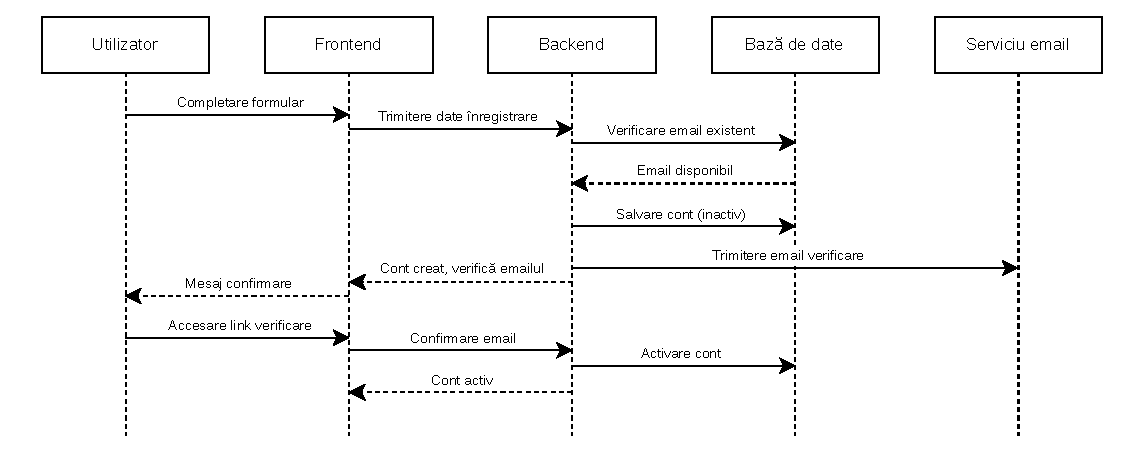
\includegraphics[width=0.8\textwidth]{pics/diagrams/sequence-registration.pdf}
    \caption{Diagramă de secvență: Înregistrarea unui cont de student}
    \label{fig:sequence-registration}
\end{figure}

\textbf{Condiție prealabilă:} utilizatorul nu are un cont existent pe platformă.

Utilizatorul accesează platforma și completează formularul de înregistrare, introducând adresa de email, parola și celelalte date necesare, sistemul validând datele introduse și verificând că adresa de email nu este deja asociată unui cont existent, returnând un mesaj de eroare corespunzător în cazul în care oricare dintre condiții nu este îndeplinită. În cazul utilizatorilor minori, este necesară și obținerea consimțământului parental, platforma trimițând automat o solicitare la adresa de email a părintelui sau tutorelui legal înainte de activarea contului, acesta devenind activ doar după primirea acordului. După validarea cu succes a tuturor datelor, sistemul trimite un email de verificare la adresa introdusă, contul devenind activ doar după confirmarea acestuia prin accesarea link-ului primit, utilizatorul putând apoi accesa toate funcționalitățile disponibile rolului de student și să parcurgă conținutul disponibil în catalog (\Cref{fig:sequence-registration}).

\textbf{Condiție ulterioară:} contul este activ și utilizatorul este autentificat în platformă.

\textbf{Scenariul 2:} Rezervarea unei sesiuni cu un profesor

\begin{figure}[htbp]
    \centering
    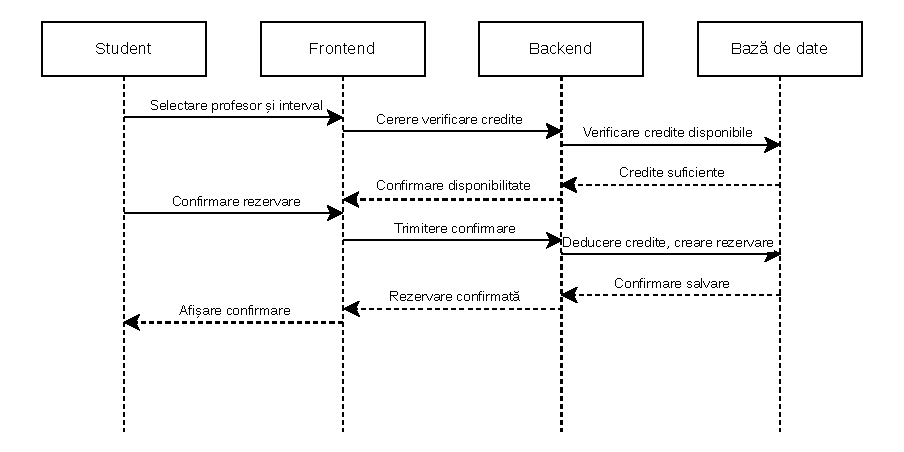
\includegraphics[width=0.8\textwidth]{pics/diagrams/sequence-booking.pdf}
    \caption{Diagramă de secvență: Rezervarea unei sesiuni}
    \label{fig:sequence-booking}
\end{figure}

\textbf{Condiție prealabilă:} studentul are un cont activ și un abonament cu credite disponibile, iar cel puțin un profesor are disponibilitate configurată.

Studentul accesează secțiunea dedicată sesiunilor și vizualizează profesorii disponibili, selectând un profesor și un interval orar din disponibilitatea acestuia, putând alege între o sesiune individuală sau una de grup în funcție de preferință și de oferta disponibilă, fiecare tip de sesiune deducând un număr diferit de credite din contul studentului. Înainte de confirmarea rezervării, sistemul verifică dacă studentul dispune de suficiente credite pentru tipul de sesiune ales. În caz contrar, îi afișează un mesaj corespunzător, nepermițându-i să finalizeze rezervarea fară a dispune de credite suficiente. La confirmarea rezervării, creditele sunt deduse automat din contul studentului, profesorul primind o notificare, iar sesiunea apărând în programul ambilor utilizatori, aceștia putând vedea detaliile complete ale rezervării din profilul lor. La momentul sesiunii, ambii participanți pot accesa camera video direct din interfața platformei, întreaga interacțiune desfășurându-se fără a fi redirecționați către o aplicație externă, asigurând o experiență unitară în cadrul sistemului (\Cref{fig:sequence-booking}).

\textbf{Condiție ulterioară:} sesiunea este rezervată, creditele sunt deduse și sesiunea este vizibilă în contul ambilor utilizatori.

\textbf{Scenariul 3: Crearea și aprobarea unui curs}

\begin{figure}[htbp]
    \centering
    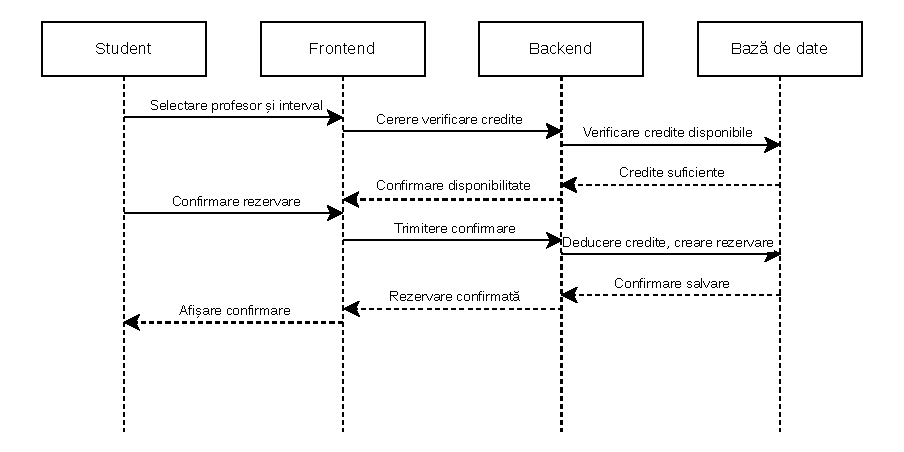
\includegraphics[width=0.8\textwidth]{pics/diagrams/sequence-course-approval.pdf}
    \caption{Diagramă de secvență: Crearea și aprobarea unui curs}
    \label{fig:sequence-course-approval}
\end{figure}

\textbf{Condiție prealabilă:} profesorul are un cont aprobat și activ pe platformă.

Profesorul accesează secțiunea de gestionare a cursurilor și creează un curs nou, completând titlul, descrierea și nivelul de dificultate, adăugând ulterior lecțiile și conținutul asociat fiecăreia, incluzând exerciții interactive de mai multe tipuri și quiz-uri cronometrate, cursul rămânând în stare de draft pe toată durata procesului de creare și putând fi editat oricând, fără a fi vizibil studenților. După finalizare, profesorul trimite cursul spre publicare, acesta intrând automat într-un flux de revizuire gestionat de administrator, care analizează conținutul și poate aproba publicarea în catalog sau poate respinge cursul adăugând note cu motivul deciziei, profesorul primind o notificare cu rezultatul și putând face modificările necesare înainte de a retrimite cursul spre revizuire. Dacă cursul este aprobat, acesta devine imediat vizibil studenților în catalog și poate fi accesat și parcurs, profesorul primind o confirmare a publicării și putând urmări de atunci înainte statistici legate de parcurgerea conținutului de către studenți (\Cref{fig:sequence-course-approval}).

\textbf{Condiție ulterioară:} cursul este publicat în catalog și accesibil studenților sau profesorul este notificat cu privire la respingere și poate efectua modificările necesare.
